\chapter{Learning from data}
\label{chap:slt}
\glsresetall

\chapterprecishere{%
  To understand God's thoughts we must study statistics, for these are the measures of His purpose.
  \par\raggedleft--- \textup{Florence Nightingale}, her diary}

As we discussed before, in this book, I focus on the problem of inferring a solution for a
predictive task from data.  In this chapter, we introduce the basic concepts of the
\gls{slt}, a general framework for predictive learning tasks.

More specifically, we discuss the \emph{inductive learning} approach, which involves
deriving general rules from specific observations.

We also formally establish the learning problem, and we define the two most common
predictive tasks: binary data classification and regression estimation.  We discuss the
optimal solutions for these tasks in an ideal (although unrealistic) scenario where the
distributions of the data are known.

Moreover, we discuss principles that guide the learning process if the distribution of
the data is unknown.  From those principles, we discuss the properties and limitations of
the learning process.

Finally, we realize those concepts for simple linear problems, explaining two basic
algorithms for the learning process: the perceptron and the maximal margin classifier.
% TODO: if regression is shown, update here with adaline and svr

\begin{mainbox}{Chapter remarks}

  \boxsubtitle{Contents}

  \startcontents[chapters]
  \printcontents[chapters]{}{1}{}
  \vspace{1em}

  \boxsubtitle{Context}

  \begin{itemize}
    \itemsep0em
    \item Inductive reasoning is the process of deriving general rules from specific
      observations.
  \end{itemize}

  \boxsubtitle{Objectives}

  \begin{itemize}
    \itemsep0em
    \item Define the learning problem and the common predictive tasks.
    \item Understand the main principles that guide the learning process.
  \end{itemize}

  \boxsubtitle{Takeaways}

  \begin{itemize}
    \itemsep0em
    \item Optimal solutions establish how good a solution can possibly be.
    \item Reducing error is not enough to guarantee a good solution.
    \item Controlling model complexity is crucial for generalization.
  \end{itemize}
\end{mainbox}

{}
\clearpage

\section{Introduction} % TODO: I don't like this title

Several problems can be addressed by techniques that utilize data in some way.  Once we focus on
one particular problem --- inductive learning ---, we need to define the scope of the
tasks we are interested in.  Let us start from the broader fields to the more specific
ones.

\Gls{ai} is a very broad field, including not only the study of algorithms
that exhibit intelligent behavior, but also the study of the behavior of intelligent
systems.  For instance, it encompasses the study of optimization methods, bio-inspired algorithms,
robotics, philosophy of mind, and many other topics.  We are interested in the subfield of
artificial intelligence that studies algorithms that exhibit some form of intelligent
behavior.

A more specific subfield of \gls{ai} is \gls{ml}, which studies algorithms that
enable computers to learn and improve their performance on a task from
experience automatically, without being explicitly programmed by a human being.

Programming a computer to play chess is a good example of the difference between
traditional \gls{ai} and \gls{ml}.  In traditional \gls{ai}, a human programmer
would write a program that contains the rules of chess and the strategies to play the game.
The algorithm might even ``search'' among the possible moves to find the best one.  In
\gls{ml}, the programmer would write a program that learns to play chess by playing
against itself, against other programs, or even from watching games played by humans.
The system would learn the rules of chess and the strategies to play the game by itself.

This field is particularly useful when the task is too complex to be solved by
traditional programming methods or when we do not know how to solve the task.
Among the many tasks that can be addressed by \gls{ml}, we can specialize even more.

Predictive learning is the \gls{ml} paradigm that focuses on making predictions about
outcomes (sometimes about the future) based on historical data.  Predictive tasks
involve predicting the value of a target variable based on the values of one or more
input variables\footnote{Descriptive learning, which is out of the scope of this book,
focuses on describing the relationships between variables in the data without the
need for a target variable.}.

Depending on the reasoning behind the learning algorithms, we can divide the learning
field into two main approaches: \emph{inductive learning} and \emph{transductive
learning}\footnote{Trasduction is the process of obtaining specific knowledge from specific
observations, and it is not the focus of this book.}.

Inductive learning involves deriving general rules from specific observations.  The
general rules can make predictions about \emph{any} new instances.  Such an approach
is exactly what we want to apply in the project methodology we described in
\cref{sec:our-approach}:  the solution is the general rule inferred from the data.

\begin{figurebox}[label=fig:learning]{Organizational chart of the learning field.}
  \centering
  \begin{tikzpicture}
    \draw[outline] (0,0) circle (30mm) node {};
    \node[below] at (0, 2.6) {artificial intelligence};
    \draw[outline] (0,-0.5) circle (25mm) node {};
    \node[below] at (0, 1.6) {machine learning};
    \draw[outline] (0,-1) circle (20mm) node {};
    \node[below] at (0, 0.5) {predictive learning};
    \draw[outline] (0,-1.5) circle (15mm) node {};
    \node[below] at (0, -1.0) {inductive learning};
  \end{tikzpicture}
  \tcblower
  Artificial intelligence studies algorithms that exhibit intelligent behavior and the
  behavior of intelligent systems.  Machine learning is a subfield of artificial
  intelligence that studies algorithms that enable computers to automatically learn from
  data.  Predictive learning, which focuses on making predictions about outcomes given
  known input data.  Inductive learning is a yet more specific type of learning that
  involves deriving general rules from specific observations.
\end{figurebox}

\Cref{fig:learning} gives us a hierarchical view of the learning field.  Alternatives ---
such as descriptive learning in opposition to predictive learning, or transductive
learning in opposition to inductive learning --- are out of the scope of this book.

Maybe the most general (and useful) framework for predictive learning is \gls{slt}.
In this chapter, we will introduce the basic concepts of this theory and discuss the
properties of the main \gls{ml} methods.

\section{The learning problem}
\label{sec:learning-problem}

Consider the set
\begin{equation}
  \label{eq:training-set}
  \big\{(\vec{x}_i, y_i) : i = 1, \dots, n \big\}
\end{equation}
where each sample $i$ is associated with a feature vector $\vec{x}_i \in \mathcal{X}$ and a target variable
$y_i \in \mathcal{Y}$.  We assume that samples are random, independent, and identically
distributed (i.i.d.) observations drawn according to $$\Prob(x, y) = \Prob(y \mid x) \Prob(x)\text{.}$$
Both distributions $\Prob(x)$ and $\Prob(y \mid x)$ are fixed but unknown.

This is equivalent to the original \gls{slt} setup stated by \textcite{Vapnik1999b}, where
a generator produces random vectors $\vec{x}$ according to a fixed but unknown
probability distribution $\Prob(x)$ and a supervisor returns an output value $y$ for every
input vector $x$ according to a conditional distribution function $\Prob(y \mid x)$, also fixed but
unknown.

Moreover, note that this setup is compatible with the idea of tidy data and 3NF (see
\cref{sub:bridge}). Of course, we assume $X, Y$ are only the measured variables (or
non-prime attributes).  In practice, it means that we set aside the keys in the learning
process.

In terms of the tables defined in \cref{sec:formal-structured-data}, any row $r$ in the
table $T = (K, H, c)$, in the desired observational unit, such that $\rowcard[r] > 0$, and
$h \in H$ the chosen target variable, we have a corresponding target $y = c(r, h)$ and a
feature vector $\vec{x}$ that corresponds to the tuple $$\big(c(r, h') : h' \in H \setminus
\left\{ h \right\}\big)\text{.}$$  Similarly, the variables $K$ that describe each unit
are set aside, as it does not make sense to infer general rules from them.

From the statistical point of view, learning problems consist of answering questions about
the distribution of the data.

\subsection{Learning tasks}

In terms of predictive learning, given the before-mentioned scenario, we can refine our
goals by tackling specific tasks\footnote{I consider tasks as well-defined subproblems of
a higher-level problem.}.

Consider a \emph{learning machine} capable of generating a set of functions, or
\emph{models}, $f(x; \theta) \equiv f_\theta(x)$, for a set of parametrizations $\theta
\in \Theta$ and such that $f_\theta : \mathcal{X} \rightarrow \mathcal{Y}$.  In a learning
task, we must choose, among all possible $f_\theta$, the one that predicts the target
variable in the best possible way.

In order to learn, we must first define the \emph{loss} (or discrepancy) $\mathcal{L}$
between the response $y$ to a given input $x$, drawn from $\Prob(x, y)$, and the
response provided by the learned function.

Then, given the \emph{risk function}
\begin{equation}
  \label{eq:risk}
  R(\theta) = \int \mathcal{L}(y, f_\theta(x))\, d\!\Prob(x, y)\text{,}
\end{equation}
the goal is to find the function $f_\theta$ that minimizes $R(\theta)$
where the only available information is the \emph{training set} given by \eqref{eq:training-set}.

This formulation encompasses many specific tasks. I focus on two of them, which I
believe are the most fundamental ones: \emph{binary data classification}\footnote{In
\gls{slt}, Vapnik calls it \emph{pattern recognition}.} and \emph{regression
estimation}\footnote{We are not talking about \emph{regression analysis}; regression
estimation is closer to the \emph{scoring} task definition by \fullcite{Zumel2019}.}.  (I
left aside the density estimation problem, once it is not addressed in the remainder of
the book.)

\subsubsection{Binary data classification task}

In this task, the output $y$ takes on
only two possible values, zero or one\footnote{Alternatively, negative class is
represented by $-1$ and positive class by $1$.} --- called the negative and the positive
class, respectively ---, and the functions $f_\theta$ are indicator
functions. Choosing the loss
\begin{equation*}
  \mathcal{L}(y, f_\theta(x)) = \begin{cases}
    0 & \text{if } y = f_\theta(x) \\
    1 & \text{if } y \neq f_\theta(x)\text{,}
  \end{cases}
\end{equation*}
the risk $\eqref{eq:risk}$ becomes the probability of
classification error.  The function $f_\theta$, in this case, is called a \emph{classifier}
and $y$ is called the \emph{label} or \emph{class}.

\subsubsection{Regression estimation task}

In this task, the output $y$ is a real value and the functions $f_\theta$ are real-valued
functions.  The loss function is the squared error
\[
  \mathcal{L}(y, f_\theta(x)) = \big(y - f_\theta(x)\big)^2\text{.}
\]
In \cref{sec:optimal-solution}, we show that the function that minimizes the risk with such
a loss function is the so-called \emph{regression}.
The estimator $f_\theta$ of the regression, in this case, is called a \emph{regressor}.

\subsection{A few remarks}

These two tasks are quite general and can be applied to a wide range of problems.  The
modeling of the task at hand and choice of the loss function are crucial to the success of
the learning process.

About these learning tasks, we can make a few remarks.

\paragraph{Supervised and semisupervised learning}
In both cases, classification and regression estimation, the learning task is to find the function
that maps the input data to the output data in the best possible way.  Although the
learning machine described generates models in a \emph{supervised} manner --- i.e., the target
is known for all samples in the training set ---, there are
alternative ways to solve the inductive learning problem, such as the \emph{semisupervised}
approach, where the model can be trained with a small subset of labeled data and a large
subset of unlabeled data --- that is, data whose outputs $y$ are unknown.

\paragraph{Generative and discriminative models}
Any learning machine produces a model that describes the relationship between the input
and output data.  This model can be generative or discriminative.  Generative models
describe the joint probability distribution $\Prob(x, y)$ and can also be used to generate new
data.  Discriminative models, on the other hand, describe the conditional probability
distribution $\Prob(y \mid x)$ directly and can only be used to make predictions. Generative models are
usually much more complex than discriminative models\footnote{Since modeling $\Prob(x, y)$
indirectly models $\Prob(y \mid x)$ and $\Prob(x)$.}, but they hold more information about
the data.  If you only
need to solve the predictive problem, prefer a discriminative model.

\paragraph{Multiclass classification}
In the binary classification task, the output $y$ is
a binary variable.  However, it is possible to have a multiclass classification task,
where  $y$ can take on more than two possible values.  Although some learning methods can
address directly the multiclass classification task, it is possible to transform the
problem into a binary classification task.  The most common method is
\emph{one-versus-all}, where we train $l$ binary classifiers, one for each class,
and the class with the highest score is the predicted class.  Another method is the
\emph{one-versus-one} method, where we train $l(l-1)/2$ binary classifiers, one for each
pair of classes, and the class with the most votes is the predicted class.
As one should expect, dealing with more than two classes is more complex than dealing
with only two classes.  If possible, prefer to deal with binary classification tasks first.

\paragraph{Number of inputs and outputs}
Note that the definition of the learning problem does not restrict the number of inputs
and outputs.  The input data can be a scalar, a vector, a matrix, or a tensor, and the
output as well.  The learning machine must be able to handle the input and output data
according to the problem.

% TODO: when discussing bias
% \paragraph{Parametric vs nonparametric models}
% The learning machine generates a set of functions $f_\theta$ where $|\theta|$ can be fixed
% or not.  If $|\theta|$ is always fixed, the model is called \emph{parametric}.  If
% $|\theta|$ is not fixed beforehand, the model is called \emph{nonparametric}.  Parametric
% models are usually simpler and faster, but they are less flexible.  In other words, it is
% up to the researcher to choose the best model ``size'' for the problem.  If the model is
% too small, it will not be able to capture the complexity of the data.  If the model is too
% large, it will be too complex, too slow to train and might overfit to the data.
% Nonparametric models are more flexible, but they usually require more data to be trained.

\section{Optimal solutions}
\label{sec:optimal-solution}

In this section, I show that the optimal solutions for the tasks of binary data
classification and regression estimation depend only on $\Prob(y \mid x)$ (i.e.
discriminative models).  This is useful
to understand how good a solution can possibly be and to derive practical solutions in the
next sections.

\subsection{Bayes classifier}

The optimal solution for the binary data classification task is the \emph{Bayes
classifier}, which minimizes the probability of classification error.  The Bayes
classifier is defined as
\begin{equation*}
  f_\text{Bayes}(x) = \argmax_{y \in \mathcal{Y}} \Prob(y \mid x)\text{.}
\end{equation*}

We can easily see that the Bayes classifier is the optimal solution for the binary data
classification task.  The probability of classification error for an arbitrary classifier
$f$ is
\begin{equation*}
  R(f) = \int \mathbb{1}_{f(x) \neq y}\, d\!\Prob(x, y) =
    \iint \mathbb{1}_{f(x) \neq y}\, d\!\Prob(y | x)\, d\!\Prob(x)\text{,}
\end{equation*}
where $\mathbb{1}_{\cdot}$ is the indicator function that returns one if the condition is
true and zero otherwise.  Let $b(x) = \Prob(y = 1 \mid x)$; we have that
\[
  \int \mathbb{1}_{f(x) \neq y}\, d\!\Prob(y | x) =
    b(x) \mathbb{1}_{f(x) = 0} + (1 - b(x)) \mathbb{1}_{f(x) = 1}\text{,}
\]
which means only one of the terms is nonzero for each $x$.  Thus, the risk is minimized by choosing
a classifier that $f(x) = 1$ if $b(x) > 1 - b(x)$ and $f(x) = 0$ otherwise.  This is the
Bayes classifier.

Consequently, the \emph{Bayes error rate}, or irreducible error, is the lowest possible loss for any
classifier in a given problem.  The Bayes error rate sums the errors of the
Bayes classifier for each class:
\begin{equation*}
  R_\text{Bayes} = \int \left[
    b(x) \mathbb{1}_{f_\text{Bayes}(x) = 0} +
    \left(1 - b(x)\right) \mathbb{1}_{f_\text{Bayes}(x) = 1}
  \right] d\!\Prob(x)\text{.}
\end{equation*}

We know that $f_\text{Bayes}(x) = 1$ if $b(x) > 0.5$ and $f_\text{Bayes}(x) = 0$ otherwise.
Thus, the Bayes error rate can be rewritten as
\begin{equation*}
  R_\text{Bayes} = \int \min\left\{ b(x), 1 - b(x) \right\}\, d\!\Prob(x)\text{.}
\end{equation*}

\begin{figurebox}[label=fig:bayes-classifier]{Bayes classifier illustration.}
  \centering
  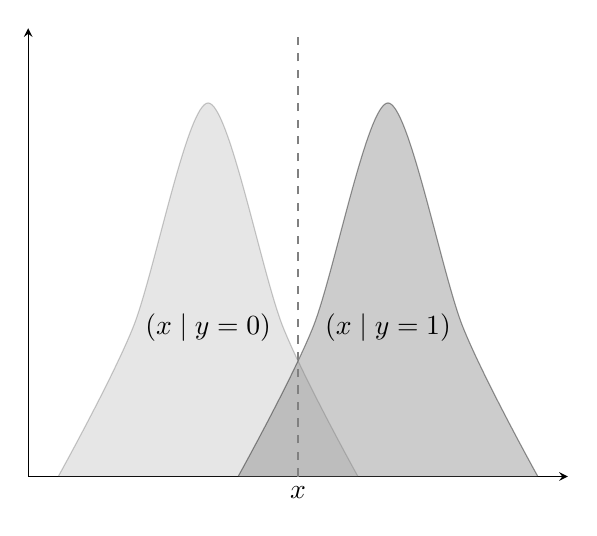
\begin{tikzpicture}
    \begin{axis}[
        ticks=none,
        axis x line=bottom,
        axis y line=left,
        xlabel={$x$},
        ymax=0.4,
        xmin=-2.2, xmax=1.4,
      ]
      % P(x|y=0)
      \addplot+[fill=gray, draw=black, opacity=0.2, smooth, mark=none] coordinates {
        (-2, 0.1) (-1.5, 0.2) (-1, 0.35) (-0.5, 0.2) (0, 0.1)
      };
      \node at (axis cs:-1, 0.2) {$\Prob(x \mid y = 0)$};
      % P(x|y=1)
      \addplot+[fill=gray, draw=black, opacity=0.4, smooth, mark=none] coordinates {
        (-0.8, 0.1) (-0.3, 0.2) (0.2, 0.35) (0.7, 0.2) (1.2, 0.1)
      };
      \node at (axis cs:0.2, 0.2) {$\Prob(x \mid y = 1)$};
      % Bayes
      \draw[dashed, gray] (axis cs:-0.4, 0) -- (axis cs:-0.4, 0.4);
    \end{axis}
  \end{tikzpicture}
  \tcblower
  The Bayes classifier is the line that separates the two classes.  The Bayes error is a
  result of the darker area in which the distributions of the classes intersect.
\end{figurebox}

\Cref{fig:bayes-classifier} illustrates the Bayes classifier and its error rate.
The vertical line represents the Bayes classifier that separates the classes the best way
possible in the space of the feature vectors $x$.  Since the distributions $\Prob(x \mid y
= 0)$ and $\Prob(x \mid y = 1)$ may intersect, there is a region where the Bayes
classifier cannot always predict the class correctly.

\subsection{Regression function}
\label{sec:regression-function}

In the regression estimation task, the goal is to approximate the optimal solution, called
\emph{regression function},
\begin{equation}
  \label{eq:regression-function}
  r(x) = \int y\, d\!\Prob(y \mid x)\text{,}
\end{equation}
that is the expected value of the target variable $y$ given the input $x$.

It is easy to show that the regression function minimizes the risk \eqref{eq:risk} with
loss
\[
  \mathcal{L}(y, r(x)) = \big(y - r(x)\big)^2\text{.}
\]
The risk functional for an arbitrary function $f$ is
\begin{multline*}
  R(f) =
    \int \big(y - f(x)\big)^2\, d\!\Prob(x, y) =\\
    \int y^2\, d\!\Prob(y) -
    2 \int f(x) \left[ \int y\, d\!\Prob(y \mid x) \right] d\!\Prob(x) +
    \int f(x)^2\, d\!\Prob(x)\text{,}
\end{multline*}
however we can substitute $r(x)$ for the inner integral and obtain
\begin{multline*}
  R(f) =
    \int y^2\, d\!\Prob(y) - 2 \int f(x) r(x)\, d\!\Prob(x) + \int f(x)^2\, d\!\Prob(x) = \\
    \int y^2\, d\!\Prob(y) + \int \left[ f(x)^2 - 2 f(x) r(x) \right]\, d\!\Prob(x)\text{.}
\end{multline*}
Once the first term is a constant, the risk is minimized by minimizing
\[
  f(x)^2 - 2 f(x) r(x)\text{.}
\]

Deriving the last expression with respect to $f(x)$ and setting it to zero, we obtain
\begin{equation*}
  \frac{d}{d f(x)} \Big[ f(x)^2 - 2 f(x) r(x) \Big] = 2 f(x) - 2 r(x) = 0 \Rightarrow
  f(x) = r(x)\text{.}
\end{equation*}

Like the Bayes classifier, the stochastic nature of the data leads to an irreducible
error in the regression estimation task.  We have that
\begin{equation*}
  R(r) = \int \big(y - r(x)\big)^2\, d\!\Prob(x, y) =
    \int y^2\, d\!\Prob(y) - \int r(x)^2\, d\!\Prob(x)\text{,}
\end{equation*}
where the first term is
\[
  \E\!\left[y^2\right] = \Var(y) + \E\!\left[y\right]^2
\]
and the second term is
\[
  \E\left[\E\!\left[y \mid x\right]^2\right] =
    \Var\!\left(\E\!\left[y \mid x\right]\right) + \E\!\left[\E\!\left[y \mid x\right]\right]^2 =
    \Var\!\left(\E\!\left[y \mid x\right]\right) + \E\!\left[y\right]^2\text{.}
\]
Thus, the irreducible error is
\[
  R(r) = \Var(y) - \Var\!\left(\E\!\left[y \mid x\right]\right) \text{.}
\]

The interpretation of the irreducible error comes from the law of the total variance:
\begin{equation*}
  \Var(y) = \E\!\left[ \Var(y \mid x) \right] + \Var\!\left(\E\!\left[y \mid x\right]\right)\text{,}
\end{equation*}
where the first term is known as the unexplained variance and the second term, as the
explained variance.  The equality $R(r) = \E\!\left[ \Var(y \mid x) \right]$
captures the idea that this variance is the intrinsic uncertainty that cannot be further
reduced.

\begin{figurebox}[label=fig:explained-unexplained-variance]{Unexplained variance is the
  error of the regression.}
  \centering
  \begin{tikzpicture}
    \begin{axis}[
        axis lines=middle,
        xlabel={$x$},
        ylabel={$y$},
        xmin=-0.2, xmax=1.5,
        ymin=-0.5, ymax=1.8,
        xtick={0, 0.5, 1},
        ytick={0, 0.5, 1},
        domain=0:1]

      \addplot[thick] {x} node[right] {$r(x) = x$};

      \addplot [draw=none, fill=gray, opacity=0.2] {x + 1} \closedcycle;
      \addplot [draw=none, fill=gray, opacity=0.2] {x - 1} \closedcycle;
      \draw[Stealth-Stealth, gray] (axis cs:0.5,0.5) -- (axis cs:0.5, 1.5) node[midway, right] {$\sigma = 1$};
      \node at (axis cs:0.5,1.3) [anchor=west] {Unexplained variance};

     \addplot[samples=2, style={dashed}] {0.5} node[midway, below, anchor=north west] {Explained variance};
    \end{axis}
  \end{tikzpicture}
  \tcblower
  Expected error of the regression function for data generated by
  $\Prob(y \mid x) \Prob(x)$ such that $\Prob(y \mid x) = \mathcal{N}(x, 1)$ and
  $\Prob(x) = \mathcal{U}(0, 1)$.  The regression function is $r(x) = x$.
\end{figurebox}

\Cref{fig:explained-unexplained-variance} illustrates the irreducible error of the
regression function for arbitrary distributions $\Prob(y \mid x)$ and $\Prob(x)$.
In this case, $\E\!\left[ \Var(y \mid x) \right] = 1$, which means that points drawn
by $\Prob(x, y)$ are distributed around the regression function $r(x)$ with a standard
deviation of one.  The explained variance is the spread of the regression across the
x-domain.

\section{ERM inductive principle}

It is very interesting to study the optimal solution for learning tasks, but in the
real-world, we do not have access to the distributions $\Prob(x)$ and $\Prob(y \mid x)$.
We must rely on the training data $(x_1, y_1), \dots, (x_n, y_n)$ to infer a solution.

In the following sections, for the sake of simplicity, let $z$ describe the pair $(x, y)$
and $L(z, \theta)$ be a generic loss function for the model $f_\theta$.  Note that the
training dataset is thus a set of $n$ i.i.d. samples $z_1, \dots, z_n$.

Since the distribution $\Prob(z)$ is unknown, the risk functional $R(\theta)$ is replaced by
the \emph{empirical risk functional}
\begin{equation}
  \label{eq:empirical-risk}
  R_n(\theta) = \frac{1}{n} \sum_{i=1}^n L(z_i, \theta)\text{.}
\end{equation}
```

Approximating $R(\theta)$ by the empirical risk functional $R_n(\theta)$ is the so-called
\gls{erm} inductive principle.  The ERM principle is the basis of the \gls{slt}.

Traditional methods, such as least squares, maximum likelihood, and maximum a posteriori, are
all realizations of the ERM principle for specific loss functions and hypothesis spaces.

\subsection{Consistency of the learning process}

One important question about the ERM principle is the consistency of the learning process.
Consistency means that, given a sufficient number of samples, the empirical risk
functional $R_n(\theta)$ converges to the true risk functional $R(\theta)$ over the
hypothesis space $\Theta$.

The consistency of the ERM principle is guaranteed by the uniform (two-sided)
convergence\footnote{Actually, only a weaker one-sided uniform convergence is needed; consult a
detailed explanation in chapter 2 of \fullcite{Vapnik1999b}.  The equivalence is a
consequence of the key theorem of learning proved by Vapnik and Chervonenkis in 1989 and
later translated to English in \fullcite{Vapnik1991}.} of the empirical risk functional
$R_n(\theta)$ to the true risk functional $R(\theta)$ over the hypothesis space $\Theta$.
The uniform convergence is defined as
\[
  \lim_{n \to \infty} \Prob\!\left(
    \sup_{\theta \in \Theta} \Big| R_n(\theta) - R(\theta) \Big| > \epsilon
  \right) = 0\text{.}
\]

\subsection{Rate of convergence}

Beyond consistency, it is also useful to understand the rate at which $R_n(\theta)$
converges to $R(\theta)$ as the sample size $n$ increases.  It is possible for a learning
machine to be consistent but have a slow convergence rate, which means that a large number of
samples is needed to achieve a good solution.

The asymptotic rate of convergence of the empirical risk functional $R_n(\theta)$ is
fast if, for any $n > n_0$, the exponential bound
\[
  \Prob\!\big(R(\theta_n) - R(\theta) > \epsilon\big) < \exp\!\left( - c n \epsilon^2 \right)
\]
holds true, where $c$ is a positive constant.

\subsection{VC entropy}

Let $L(z, \theta)$, $\theta \in \Theta$, be a set of bounded loss functions, i.e.
\[
  \left| L(z, \theta) \right| < M\text{,}
\]
for some constant $M$ and all $z$ and $\theta$.  One can construct $n$-dimensional vectors
\[
  l(z_1, \dots, z_n; \theta) = \big[ L(z_1, \theta), \dots, L(z_n, \theta) \big]\text{.}
\]
Once the loss functions are bounded, this set of vectors belongs to a $n$-dimensional
cube and has a finite minimal $\epsilon$-net\footnote{An $\epsilon$-net is a set of points
that are $\epsilon$-close to any point in the set.}.

Consider the quantity $N(z_1, \dots, z_n; \Theta, \epsilon)$ that counts the number of
elements of the minimal $\epsilon$-net of that set of vectors.
Once the quantity $N$ is a random variable, we can define the VC entropy as
\[
  H(n; \Theta, \epsilon) = \E\!\left[ \ln N(z_1, \dots, z_n; \Theta, \epsilon) \right]\text{,}
\]
where $z_i$ are i.i.d. samples drawn from some $\Prob(z)$.

If $L(z, \theta)$, $\theta \in \Theta$, is a set of indicator functions (i.e., the loss in a binary
classification task),  we measure the diversity of this set using the quantity $N(z_1,
\dots, z_n; \Theta)$ that counts the number of different separations of the given sample
that can be made by the functions.  In this case, the minimal $\epsilon$-net for $\epsilon < 1$
does not depend on $\epsilon$ and is a subset of the vertices of the unit cube.

A necessary and sufficient condition for uniform convergence is
\begin{equation}
  \label{eq:uniform-convergence}
  \lim_{n \to \infty} \frac{H(n; \Theta, \epsilon)}{n} = 0\text{,}
\end{equation}
for all $\epsilon > 0$.

The VC entropy measures the complexity of the hypothesis space $\Theta$.  The intuition
behind the need for a decreasing VC entropy with increasing numbers of observations is
related to the nonfalsifiability of the learning machine.  For instance, the set of
functions that can always separate the training data perfectly (contains all the vertices
of the cube) is nonfalsifiable because
it implies that the minimum of the empirical risk is zero independently of the value of
the true risk.

\subsection{Growing function and VC dimension}
\label{sub:vc-dimension}

It turns out that we can guarantee both the uniform convergence and the fast rate of
convergence independently of $\Prob(z)$.  Actually,
\[
  \lim_{n \to \infty} \frac{G(n; \Theta)}{n} = 0
\]
is the necessary and sufficient condition, where
\[
  G(n; \Theta) = \ln \sup_{z_1, \dots, z_n} N(z_1, \dots, z_n; \Theta)\text{,}
\]
is the \emph{growth function} of the hypothesis space $\Theta$.

\textcite{Vapnik1968}\footfullcite{Vapnik1968} showed that the growth function either
satisfies
\[
  G(n; \Theta) = n \ln 2
\]
or is bounded by
\[
  G(n; \Theta) \leq h \left( \ln \frac{n}{h} + 1 \right)\text{,}
\]
where $h$ is an integer.  Thus, the growth function is either linear or logarithmic in
$n$.  In the first case, we say that the \emph{VC dimension} of the hypothesis space is
infinite, and in the second case, the VC dimension is $h$.

A finite VC dimension is enough to imply both consistency and a fast rate of convergence.

\subsubsection{Intuitions about the VC dimension}
\label{sub:vc-dimension-intuition}

% A figure with lines separating separating points in a plane
\begin{figurebox}[label=fig:vc-dimension]{VC dimension of a set of lines in the plane.}
  \centering
  \begin{tikzpicture}
    \begin{axis}[
        axis lines=middle,
        xmin=-1, xmax=1,
        ymin=-1, ymax=1,
        xtick={0},
        ytick={0},
        domain=-1:1]

      \addplot[only marks, mark=*, mark size=2pt] coordinates {
        (-0.5, 0.3) (-0.3, -0.5) (0.7, -0.5)
      };

      % diagonal lines separating points
      \addplot[dashed] {x} node[right] {$\theta_1$};
      \addplot[dashed] {-x} node[right] {$\theta_2$};
      \addplot[dashed] {-0.3} node[right] {$\theta_3$};

    \end{axis}
  \end{tikzpicture}
  \tcblower
  The VC dimension of the lines in the plane is equal to 3, since a line can shatter 3
  points in all 8 possible ways, but not four points.
\end{figurebox}

For a set of indicator functions, the VC dimension is the maximum number of vectors that
can be \emph{shattered} by the functions.  If, for any $n$, there is a set of $n$
vectors that can be shattered by the functions, the VC dimension is infinite.
We say that $h$ vectors can be shattered if they can be separated into two classes in all
$2^h$ possible ways.  \Cref{fig:vc-dimension} illustrates the VC dimension of a set of
lines in the plane.

\begin{figurebox}[label=fig:vc-sin]{High-frequency sine wave functions have an infinite VC dimension.}
  \centering
  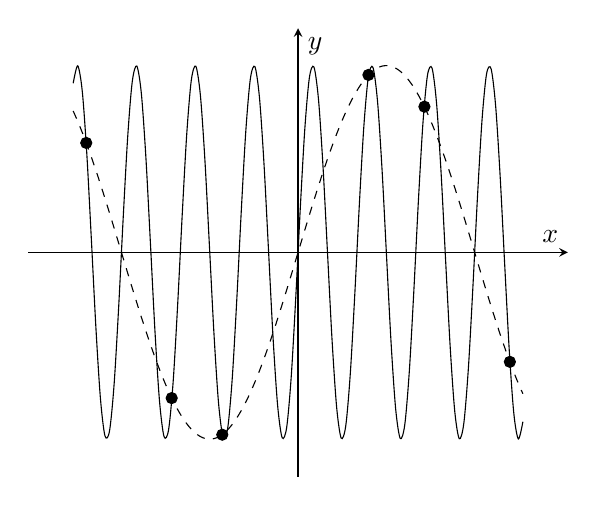
\begin{tikzpicture}
    \begin{axis}[
        axis lines=middle,
        xlabel={$x$},
        ylabel={$y$},
        xmin=-1.2, xmax=1.2,
        ymin=-1.2, ymax=1.2,
        xtick={0},
        ytick={0},
        domain=-1:1,
        samples=100]

      \addplot[smooth] {sin(deg(24 * x))};
      \addplot[dashed, smooth] {sin(deg(4 * x))};

      \addplot[only marks, mark=*, mark size=2pt] coordinates {
        (-0.942, 0.586) (-0.562, -0.780) (-0.337, -0.976)
        (0.313, 0.950) (0.562, 0.780) (0.942, -0.586)
      };
    \end{axis}
  \end{tikzpicture}
  \tcblower
  High-frequency sine waves approximate any set of points well, even though they may come
  from a low-frequency sine wave or any other function.
\end{figurebox}

One misconception about the VC dimension is that it is related to the number of parameters
of the model.  The VC dimension is actually related to the complexity of the hypothesis space, not
to the number of parameters.  For instance, the VC dimension of functions
\[
  f(z; \theta) = \mathbb{1}_{\sin \theta x > 0}
\]
is infinite, even though the parameter $\theta$ is a scalar.  See \cref{fig:vc-sin}.
By increasing the frequency $\theta$ of the sine wave, the function can approximate any set
of points.

This opens remarkable opportunities to find good solutions containing a huge number of
parameters\footnote{Sometimes, like in a linear model, the number of parameters is
proportional to the number of dimensions of the feature vector.} but with a finite VC
dimension.  % TODO: discuss non-parametric here?

\section{SRM inductive principle}

The \gls{erm} principle is a powerful tool to study the generalization ability of the
learning process.  By generalization ability, we mean the ability of the learning machine
to predict the output of new data that was not seen during the training process.  However,
it relies on the hypothesis that the number of samples tends to infinity.

In fact, \textcite{Vapnik1999b}\footfullcite{Vapnik1999b} summarizes the bounds for the
generalization ability of learning machines in the following way\footnote{ For the sake of
the arguments, we consider only the expression for bounded losses and an hypothesis space
with infinite number of functions.  Rigorously, the loss function may not be bounded;
consult the original work for the complete expressions.}:
\begin{equation}
  \label{eq:generalization-bound}
  R(\theta_n) \leq R_n(\theta_n) + \frac{B \mathcal{E}}{2} \left(
    1 + \sqrt{1 + \frac{4 R_n(\theta_n)}{B \mathcal{E}}}
  \right)\text{,}
\end{equation}
with
\[
  \mathcal{E} = 4 \frac{
    h \left( \ln \frac{2 n}{h} + 1 \right) - \ln \frac{\eta}{4}
  }{n}\text{,}
\]
where $B$ is the upper bound of the loss function, $h$ is the VC dimension of the
hypothesis space, $n$ is the number of samples.  The term $\eta$ is the confidence level,
i.e., the inequality holds with probability $1 - \eta$.

It is easy to see that as the number of samples $n$ increases, the empirical risk
$R_n(\theta_n)$ approaches the true risk $R(\theta_n)$.  Also, the greater the VC
dimension $h$, the greater the term $\mathcal{E}$, decreasing the generalization ability
of the learning machine.

In other words, if $\nicefrac{n}{h}$ is small, a small empirical risk does not guarantee a small value
for the actual risk.  A consequence is that we need to minimize both terms of the
right-hand side of the inequality \cref{eq:generalization-bound} to achieve a good
generalization ability.

% A table comparing overfit and underfit and the empirical risk and confidence interval
\begin{tablebox}[label=tab:overfit-underfit]{Overfitting and underfitting.}
  \centering
  \begin{tabular}{lll}
    \toprule
    \textbf{Problem} & \textbf{Empirical risk} & \textbf{Confidence interval} \\
    \midrule
    Underfitting & High & Low \\
    Overfitting & Low & High \\
    \bottomrule
  \end{tabular}
  \tcblower
  Two problems that can arise in the learning process are underfitting and overfitting.
  Underfitting occurs when the model is too simple (low VC dimension) and cannot capture
  the complexity of the training data (high empirical risk).  Overfitting occurs when the
  model is too complex (high VC dimension increases the confidence interval) and fits the
  training data almost perfectly (low empirical risk).
\end{tablebox}

Failure to balance the optimization of these terms leads to two problems: underfitting and
overfitting.  \Cref{tab:overfit-underfit} summarizes the problems.

The \gls{srm} principle consists of minimizing both the empirical risk (optimizing the
parameters of the model) and the confidence interval (controlling VC dimension).

Let $\Theta_k \subset \Theta$ and
\[
  S_k = \left\{ L(z, \theta) : \theta \in \Theta_k \right\}
\]
such that
\[
  S_1 \subset S_2 \subset \dots \subset S_n \subset \dots\text{,}
\]
satisfying
\[
  h_1 \leq h_2 \leq \dots \leq h_n \leq \dots\text{,}
\]
where $h_k$ is the finite VC dimension\footnote{Note that the VC dimension considering the
whole set $\Theta$ might be infinite.  Moreover, in the original formulation, the sets
$S_k$ also need to satisfy some bounds; read more in chapter 4 of \fullcite{Vapnik1999b}.}
of each set $S_k$.  This is called an \emph{admissible structure}.

\begin{figurebox}[label=fig:srm-tradeoff]{SRM trade-off.}
  \centering
  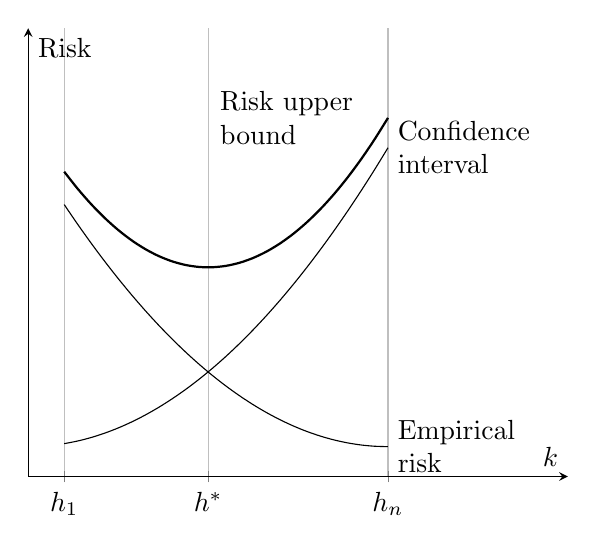
\begin{tikzpicture}
    \begin{axis}[
        axis lines=middle,
        xlabel={$k$},
        ylabel={Risk},
        ytick={0},
        yticklabels={},
        xtick={0.1, 0.5, 1},
        xticklabels={$h_1$, $h^*$, $h_n$},
        grid=both,
        xmin=0, xmax=1.5,
        ymin=0, ymax=1.5,
        domain=0.1:1]

      \addplot[smooth] {(x - 1)^2 + 0.1} node[right, text width=2cm] {Empirical risk};
      \addplot[smooth] {x^2 + 0.1} node[right, text width=2cm] {Confidence interval};
      \addplot[smooth, thick] {x^2 + (x - 1)^2 + 0.2} node[left, text width=2cm] {Risk upper bound};

    \end{axis}
  \end{tikzpicture}
  \tcblower
  The upper bound of the risk is the sum of the empirical risk and the confidence
  interval.  The smallest bound is found for some $k^*$ in the admissible structure.
\end{figurebox}

Given the observations $z_1, \dots, z_n$, the \gls{srm} principle chooses a function
$L(z, \theta_n^k)$ that minimizes the empirical risk $R_n(\theta_n^k)$ in the subset
$S_k$ for which the guaranteed risk --- upper bound considering the confidence interval
--- is minimal.  This is a trade-off between the quality of the approximation and the
complexity of the approximating function --- see \cref{fig:srm-tradeoff}.

\subsection{Bias invariance trade-off}

The trade-off that the \gls{srm} principle deals with is the general case of the so-called
\emph{bias-variance trade-off}.  The bias-variance trade-off is a well-known concept in
machine learning that describes the relationship between different kinds of errors a model
can have.

The \emph{bias error} comes from failure to capture relevant relationships between features
and target outputs.  The \emph{variance error} comes from erroneously modeling the random
noise in the training data.

The terms bias and variance (and the irreducible error) are clearly illustrated by
studying the particular regression estimation task.

Consider a learning machine that produces a function $\hat{f}(x; D)$ based on the
training set $$D = \big\{(x_1, y_1), \dots, (x_n, y_n)\big\}$$ such that
\[
  y_i = f(x_i) + \epsilon\text{,}
\]
for a fixed function $f$ and a random noise $\epsilon$ with zero mean and variance
$\sigma^2$, where $x_i$ are i.i.d. samples drawn from some distribution $\Prob(x)$.

Also, consider that $\bar{f}(x)$ is the expected value of the function $\hat{f}(x; D)$
over all possible training sets $D$, i.e.
\[
  \bar{f}(x) = \int \hat{f}(x; D)\, d\!\Prob(D)\text{.}
\]
(Note that the models themselves are the random variable we are studying here.)

For any model $\hat{f}$, the expected (squared) error for a particular sample $(x, y)$,
$\E_D\!\left[ \big( y - \hat{f}(x; D) \big)^2 \right]$, is
\begin{align}
  \notag \int \big( y - \hat{f}(x) \big)^2\, d\!\Prob(D, \epsilon)
    &= \int \big( y - f(x) + f(x) - \hat{f}(x) \big)^2\, d\!\Prob(D, \epsilon) \\
    &= \label{eq:term1}\int \big( y - f(x) \big)^2\, d\!\Prob(D) \\
    &+ \label{eq:term2}\int \big( f(x) - \hat{f}(x) \big)^2\, d\!\Prob(D) \\
    &+ \label{eq:term3}2 \int \big( y - f(x) \big)\,\big( f(x) - \hat{f}(x) \big)\, d\!\Prob(D, \epsilon)\text{.}
\end{align}

The term \eqref{eq:term1} is the irreducible error:
\begin{equation}
  \label{eq:irreducible-error}
  \int \big( y - f(x) \big)^2\, d\!\Prob(D) =
  \int \big( f(x) + \epsilon - f(x) \big)^2\, d\!\Prob(D) =
  \int \epsilon^2\, d\!\Prob(D) = \sigma^2\text{.}
\end{equation}
As the best solution is $f$ itself, the error that comes from the noise is unavoidable.

The term \eqref{eq:term3} is null:
\begin{multline*}
  \int \big( y - f(x) \big)\,\big( f(x) - \hat{f}(x) \big)\, d\!\Prob(D, \epsilon) =
  \int \epsilon\,\big( f(x) - \hat{f}(x) \big)\, d\!\Prob(D, \epsilon) = \\
  \cancelto{0}{\int \epsilon\, d\!\Prob(\epsilon)} \int \big( f(x) - \hat{f}(x) \big)\, d\!\Prob(D) = 0\text{,}
\end{multline*}
since $\Prob(D)$ and $\Prob(\epsilon)$ are independent and $\E[\epsilon] = 0$ by
definition.

We can apply a similar strategy to analyze the term \eqref{eq:term2}:
\begin{align}
  \notag \int \big( f(x) - \hat{f}(x) \big)^2\, d\!\Prob(D)
    &= \int \big( f(x) - \bar{f}(x) + \bar{f}(x) - \hat{f}(x) \big)^2\, d\!\Prob(D) \\
    &= \label{eq:term4}\int \big( f(x) - \bar{f}(x) \big)^2\, d\!\Prob(D) \\
    &+ \label{eq:term5}\int \big( \bar{f}(x) - \hat{f}(x) \big)^2\, d\!\Prob(D) \\
    &+ \label{eq:term6}2 \int \big( f(x) - \bar{f}(x) \big)\,\big( \bar{f}(x) - \hat{f}(x) \big)\, d\!\Prob(D)\text{.}
\end{align}

Now, the term \eqref{eq:term6} is also null:
\begin{multline*}
  \int \big( f(x) - \bar{f}(x) \big)\,\big( \bar{f}(x) - \hat{f}(x; D) \big)\, d\!\Prob(D) = \\
  \big( f(x) - \bar{f}(x) \big) \int \big( \bar{f}(x) - \hat{f}(x; D) \big)\, d\!\Prob(D) = \\
  \big( f(x) - \bar{f}(x) \big) \cancelto{0}{\left( \bar{f}(x) - \int \hat{f}(x; D)\, d\!\Prob(D) \right)} = 0\text{,}
\end{multline*}
since $\bar{f}(x)$ is the expected value of $\hat{f}(x; D)$.

The term \eqref{eq:term4} does not depend on the training set, so
\begin{equation}
  \label{eq:bias}
  \int \big( f(x) - \bar{f}(x) \big)^2\, d\!\Prob(D) =
  \big( f(x) - \bar{f}(x) \big)^2\text{.}
\end{equation}
This term is the square of the bias of the models.

The term \eqref{eq:term5} is the variance of the function $\hat{f}(x; D)$:
\begin{multline}
  \label{eq:model-variance}
  \int \big( \bar{f}(x) - \hat{f}(x; D) \big)^2\, d\!\Prob(D) =\\
  \E_D\!\left[ \big( \bar{f}(x) - \hat{f}(x; D) \big)^2 \right] =
  \Var_D\!\left( \hat{f}(x; D) \right)\text{.}
\end{multline}

Finally, putting all together --- i.e.  \cref{eq:irreducible-error,eq:bias,eq:model-variance}
---, we have that the expected error for a particular sample $(x, y)$ is
\[
  \E_D\!\left[ \big( y - \hat{f}(x; D) \big)^2 \right] =
    \sigma^2 +
    \big( f(x) - \E\!\left[ \hat{f}(x; D) \right] \big)^2 +
    \Var_D\!\left( \hat{f}(x; D) \right)\text{.}
\]

The irreducible error is the regression error that cannot be reduced by any model --- see
\cref{sec:regression-function}.  The bias error is the error that one expects from the
model acquired by the learning machine and that we observe in the training data --- i.e.
the empirical risk.  The variance error, which does not depend on the real function $f$
but on the models the learning machine can generate, is the error that comes from how
different the models can be from each other --- i.e. the confidence interval that comes from
the VC dimension.

\subsection{Regularization}

Also related to the \gls{srm} principle is the concept of \emph{regularization}.
Regularization encourages models to learn robust patterns within the data rather than
memorizing it.

Regularization techniques usually modify the loss by adding a penalty term that
depends on the complexity of the model.  So, instead of minimizing the empirical risk
$R_n(\theta)$, the learning machine minimizes the regularized empirical risk
\[
  R_n(\theta) + \lambda \Omega(\theta)\text{,}
\]
where $\Omega(\theta)$ is the complexity of the model and $\lambda$ is a hyperparameter
that controls the trade-off between the empirical risk and the complexity.
Note that the regularization term acts as a proxy for the confidence interval in the
\gls{srm} principle.  However, regularization is often justified by common sense or
intuition, rather than by strong theoretical arguments.

Other approaches that indirectly control the complexity of the model --- such as early
stopping, dropout, ensembles, and pruning --- are often called implicit regularization.

\section{Linear problems}

To realize the concepts of the \gls{srm} principle in practice, we consider linear
classification tasks.

For the examples in the following subsections, we use the datasets for the AND
and the XOR problem --- see \cref{tab:and-xor}.
The AND problem is linearly separable, while the XOR problem is not.

\begin{tablebox}[label=tab:and-xor]{AND and XOR datasets.}
  \centering
  \begin{minipage}{0.45\textwidth}
    \centering
    \rowcolors{2}{black!10!white}{}
    \begin{tabular}{ccc}
      \toprule
      $x_1$ & $x_2$ & $y = x_1 \land x_2$ \\
      \midrule
      0 & 0 & 0 \\
      0 & 1 & 0 \\
      1 & 0 & 0 \\
      1 & 1 & 1 \\
      \bottomrule
    \end{tabular}
  \end{minipage}
  \begin{minipage}{0.45\textwidth}
  \centering
  \rowcolors{2}{black!10!white}{}
  \begin{tabular}{ccc}
    \toprule
    $x_1$ & $x_2$ & $y = x_1 \oplus x_2$ \\
    \midrule
    0 & 0 & 0 \\
    0 & 1 & 1 \\
    1 & 0 & 1 \\
    1 & 1 & 0 \\
    \bottomrule
  \end{tabular}
  \end{minipage}
  \tcblower
  The AND and XOR datasets are binary classification datasets where the output $y$ is the
  ``logical AND'' and the ``exclusive OR'' of the inputs $x_1$ and $x_2$, i.e.,
  $y = x_1 \land x_2$ and $y = x_1 \oplus x_2$.
\end{tablebox}

We show two learning machines that implement the \gls{srm} principle in different ways:
\begin{itemize}
  \itemsep0em
  \item The perceptron, which fixes the complexity of the model and tries to minimize the
    empirical risk; and
  \item The maximal margin classifier, which fixes the empirical risk --- in this case,
    zero -- and tries to minimize the confidence interval.
\end{itemize}

\subsection{Perceptron}
\label{sub:perceptron}

The perceptron is a linear classifier that generates a hyperplane that separates the
classes in the feature space.  It is a parametric model, and the learning process minimizes the empirical risk
by adjusting its fixed set of parameters.

\begin{defbox}{Parametric model}{parametric}
  If the learning machine generates a set of functions $f_\theta$ where the number of
  parameters $|\theta|$ is always fixed, the models are called \emph{parametric}.
\end{defbox}

Parametric models are usually simpler and faster to fit, but they are less flexible.  In
other words, it is up to the researcher to choose the best model ``size'' for the problem.
If the model is too small, it will not be able to capture the complexity of the data.  If
the model is too large, it tends to be too complex, too slow to train, and might overfit to
the data.  Note, however, that the VC dimension and number of parameters are not the same
thing --- consult \cref{sub:vc-dimension-intuition}.

The perceptron model (with two inputs) is
\begin{equation*}
  f(x_1, x_2; \vec{w} = \left[w_0, w_1, w_2\right]) = u(w_0 + w_1 x_1 + w_2 x_2)\text{,}
\end{equation*}
where $u$ is the Heaviside step function
\begin{equation*}
  u(x) = \begin{cases}
    1 & \text{if } x > 0\text{,} \\
    0 & \text{otherwise.}
  \end{cases}
\end{equation*}
The parameters $\theta = \vec{w}$ are called the weights of the perceptron.
The equation $\vec{w} \cdot \vec{x} = 0$, where $\vec{x} = [1, x_1,
x_2]$, is the equation of a hyperplane.

\begin{figurebox}[label=fig:perceptron-and]{Perceptron decision boundaries in the AND dataset.}
  \centering
  \begin{tikzpicture}
    \begin{axis}[
        axis x line=bottom,
        axis y line=left,
        xlabel={$x_1$},
        ylabel={$x_2$},
        width=0.6\textwidth,
        height=0.6\textwidth,
        xtick={0, 1},
        ytick={0, 1},
        xmin=-0.5, xmax=1.5,
        ymin=-0.5, ymax=1.5,
      ]
      \addplot+[only marks, mark=-, color=black, mark size=3pt] coordinates {
        (0, 0) (0, 1) (1, 0)
      };
      \addplot+[only marks, mark=+, color=black, mark size=3pt] coordinates {
        (1, 1)
      };
      \addplot+[domain=0:1.5, mark=none, black, thick] {1.1 - 0.6 * x};
    \end{axis}
  \end{tikzpicture}
  \tcblower
  The perceptron assumes that the classes are linearly separable.
  The hyperplane that separates the classes comes from the weights of the model.
  In this case, $w_0 = -1.1$, $w_1 = 0.6$, and $w_2 = 1$.
\end{figurebox}

In \cref{fig:perceptron-and}, we show the hyperplane (in this case, a line) that the model
with weights $\vec{w} = [-1.1, 0.6, 1]$ generates in this feature space.
As one can see, the classes are linearly separable, and the perceptron model classifies
the dataset correctly; see \cref{tab:and-perceptron}.

\begin{tablebox}[label=tab:and-perceptron]{Truth table for the predictions of the perceptron in the AND dataset.}
  \centering
  \rowcolors{2}{black!10!white}{}
  \begin{tabular}{ccc|cc}
    \toprule
    $x_1$ & $x_2$ & $y$ & $-1.1 + x_1 + x_2$ & $\hat{y}$ \\
    \midrule
    0 & 0 & 0 & -1.1 & 0 \\
    0 & 1 & 0 & -0.1 & 0 \\
    1 & 0 & 0 & -0.5 & 0 \\
    1 & 1 & 1 & 0.5 & 1 \\
    \bottomrule
  \end{tabular}
  \tcblower
  The perceptron model with parameters $w_0 = 1.1$, $w_1 = -1$, and $w_2 = -1$
  classifies the AND dataset correctly.
\end{tablebox}

\begin{figurebox}[label=fig:perceptron-xor]{Perceptron decision boundaries in the XOR
  dataset.}
  \centering
  \begin{tikzpicture}
    \begin{axis}[
        axis x line=bottom,
        axis y line=left,
        xlabel={$x_1$},
        ylabel={$x_2$},
        width=0.6\textwidth,
        height=0.6\textwidth,
        xtick={0, 1},
        ytick={0, 1},
        xmin=-0.5, xmax=1.5,
        ymin=-0.5, ymax=1.5,
      ]
      \addplot+[only marks, mark=-, color=black, mark size=3pt] coordinates {
        (0, 0) (0, 1) (1, 0)
      };
      \addplot+[only marks, mark=+, color=black, mark size=3pt] coordinates {
        (1, 1)
      };
      \addplot+[domain=0:1.5, mark=none, black, thick] {-0.5 + x};
    \end{axis}
  \end{tikzpicture}
  \tcblower
  The XOR dataset is not linearly separable.
  The hyperplane that separates the classes comes from the weights of the model.
  In this case, $w_0 = -0.5$, $w_1 = 1$, and $w_2 = -1$.
  There is no way to classify the XOR dataset correctly with a perceptron.
\end{figurebox}

In \cref{fig:perceptron-xor}, we show the hyperplane that the model $\vec{w} = [-0.5, 1, -1]$
generates for the XOR dataset.  As one can see, the perceptron model fails to solve the
task since there is no single decision boundary that can classify this data.

\begin{tablebox}[label=tab:xor-perceptron]{Truth table for the predictions of the perceptron in the XOR dataset.}
  \centering
  \rowcolors{2}{black!10!white}{}
  \begin{tabular}{ccc|cc}
    \toprule
    $x_1$ & $x_2$ & $y$ & $-0.5 + x_1 - x_2$ & $\hat{y}$ \\
    \midrule
    0 & 0 & 0 & -0.5 & 0 \\
    0 & 1 & 1 & -1.5 & 0 \\
    1 & 0 & 1 & 0.5 & 1 \\
    1 & 1 & 0 & -0.5 & 0 \\
    \bottomrule
  \end{tabular}
  \tcblower
  The perceptron model with parameters $w_0 = -0.5$, $w_1 = 1$, and $w_2 = -1$
  fails to classify the XOR dataset correctly --- as any other perceptron would do.
\end{tablebox}

It is easy to see that there are an infinite number of hyperplanes that can separate the
classes in the AND dataset.  The training procedure of the perceptron is a simple
algorithm that adjusts the weights of the model to find one of these hyperplanes ---
effectively minimizing the empirical risk.  The algorithm updates the weights iteratively
for each sample that is misclassified, repeating the samples as many times as necessary.
It stops when all samples are correctly classified.

For a binary classification problem and a perceptron with weights $\vec{w}$, there are 4
situations for a given sample $\vec{x}$ and $y$:
\begin{enumerate}
  \itemsep0em
  \item $y = 0$ and $u(\vec{w} \cdot \vec{x})= 0$;
  \item $y = 0$ and $u(\vec{w} \cdot \vec{x})= 1$;
  \item $y = 1$ and $u(\vec{w} \cdot \vec{x})= 0$;
  \item $y = 1$ and $u(\vec{w} \cdot \vec{x})= 1$.
\end{enumerate}

By definition, the algorithm must update the weights when situation 2 or 3 occurs.
Let $e = y - u(\vec{w} \cdot \vec{x})$ be the error of the model for a given sample.

In situation 2, we have that $\vec{w} \cdot \vec{x} > 0$ which means that the angle
$\alpha$ between the vectors $\vec{w}$ and $\vec{x}$ is less than $90^\circ$, since
$\|\vec{w}\|\|\vec{x}\|\cos\alpha > 0 \implies \cos\alpha > 0 \implies \alpha <
90^\circ$.  To increase the angle between the vectors, we can subtract $\eta\vec{x}$ from
$\vec{w}$, for some small $\eta > 0$ --- see \cref{fig:perceptron-w2}.  The error
here is $e = -1$.

\begin{figurebox}[label=fig:perceptron-w2]{Angle between $\vec{w}$ and $\vec{x}$ in a positive output.}
  \centering
  \begin{tikzpicture}
    \draw[-Stealth] (0, 0) -- (2, 0) node[right] {$\vec{x}$};
    \draw[-Stealth] (0, 0) -- (1, 1.8) node[right] {$\vec{w}$};
    \draw[-Stealth, dashed] (1, 1.8) -- (-0.4, 1.8) node[above] {$-\eta\vec{x}$};
    \draw[-Stealth, thick, gray] (0, 0) -- (-0.4, 1.8) node[left] {$\vec{w}'$};
    \draw (0.4, 0) arc (0:59:0.4) node[right] {$\alpha$};
  \end{tikzpicture}
  \tcblower
  A positive output for the perceptron with weights $\vec{w}$ and input $\vec{x}$ means
  that the angle between the vectors is less than $90^\circ$.  To increase the angle
  between the vectors, we can subtract $\eta\vec{x}$ from $\vec{w}$, for some small $\eta
  > 0$.
\end{figurebox}

In situation 3, we have that $\vec{w} \cdot \vec{x} < 0$ which means that the
angle $\alpha$ between the vectors $\vec{w}$ and $\vec{x}$ is greater than $90^\circ$,
since $\|\vec{w}\|\|\vec{x}\|\cos\alpha < 0 \implies \cos\alpha < 0 \implies \alpha > 90^\circ$.
To decrease the angle between the vectors, we can add $\eta\vec{x}$ to $\vec{w}$, for
some small $\eta > 0$ --- see \cref{fig:perceptron-w3}.  Now, the error is $e = 1$.

\begin{figurebox}[label=fig:perceptron-w3]{Angle between $\vec{w}$ and $\vec{x}$ in a negative output.}
  \centering
  \begin{tikzpicture}
    \draw[-Stealth] (0, 0) -- (2, 0) node[right] {$\vec{x}$};
    \draw[-Stealth, thick, gray] (0, 0) -- (1, 1.8) node[right] {$\vec{w}'$};
    \draw[-Stealth, dashed] (-0.4, 1.8) -- (1, 1.8) node[above] {$\eta\vec{x}$};
    \draw[-Stealth] (0, 0) -- (-0.4, 1.8) node[left] {$\vec{w}$};
    \draw (0.4, 0) arc (0:101:0.4) node[above] {\phantom{a }$\alpha$};
  \end{tikzpicture}
  \tcblower
  A negative output for the perceptron with weights $\vec{w}$ and input $\vec{x}$ means
  that the angle between the vectors is greater than $90^\circ$.  To decrease the angle
  between the vectors, we can add $\eta\vec{x}$ to $\vec{w}$, for some small $\eta
  > 0$.
\end{figurebox}

From those observations, we can derive a general update rule
\[
  \vec{w}' = \vec{w} + \eta e \vec{x}\text{,}
\]
where $\eta$ is a small positive number that controls the step size of the algorithm.
Note that this rule works even for cases 1 and 4, where the error is zero.

The algorithm converges given $\eta$ sufficiently small and the dataset is linearly
separable.  Note that the algorithm does not make any effort to reduce the confidence
interval.

The perceptron is (possibly) the simplest artificial neural network.  More complex
networks can be built by stacking perceptrons in layers and adding non-linear activation
functions.  The training strategies for those networks are usually based on reducing the
empirical risk using the gradient descent algorithm while controlling the complexity of
the model with regularization techniques\footnote{To counterbalance the potential
``excess'' of neurons, techniques like $l_2$ regularization ``disable'' some neurons by
pressuring their weights to zero.}.  Consult \cref{sec:mlp}.

% TODO: adaline for regression

\subsection{Maximal margin classifier}

We saw that the perceptron tries to minimize the empirical risk, but it makes no effort to
reduce the confidence interval.  A different approach would be to fix the empirical risk
--- in our case, assuming that the classes are linearly separable, to fix it to zero --- and
minimize the confidence interval.

The confidence interval is an increasing function
\[
  \Omega\!\left(\frac{h}{n}\right)\text{,}
\]
where $h$ is the VC dimension of the hypothesis space and $n$ is the number of samples.
Since the number of training samples $n$ is fixed and finite (sometimes even small), we
can minimize the confidence interval by minimizing the VC dimension $h$.

In the case of the perceptron, since it can generate any hyperplane, the VC dimension is
$h = d + 1$, where $d$ is the number of dimensions of the feature space --- consult
\cref{sub:vc-dimension-intuition}.

Before we dive into the classifier that minimizes the confidence interval, consider the
following property.  \textcite{Vapnik1999b}\footfullcite{Vapnik1999b} state that a
$\Delta$-margin separating hyperplane is the hyperplane
\[
  (\vec{w} \cdot \vec{x}) - b = 0\text{, } \|\vec{w}\| = 1\text{,}
\]
such that classifies vector $\vec{x}$ as
\[
  y = \begin{cases}
    1 & \text{if } (\vec{w} \cdot \vec{x}) - b \geq \Delta\text{,} \\
    -1 & \text{if } (\vec{w} \cdot \vec{x}) - b \leq -\Delta\text{.}
  \end{cases}
\]
Given that vectors $\vec{x} \in \mathbb{R}^d$ belong to a (hyper)sphere of radius $R$, the
VC dimension of the $\Delta$-margin separating hyperplane is
\[
  h \leq \min\left(\left\lfloor \frac{R^2}{\Delta^2} \right\rfloor, d\right) + 1\text{,}
\]
which can be less than $d + 1$.

From that property, to minimize the confidence interval, we can maximize the margin
$\Delta$ of the hyperplane.  The \emph{maximal margin classifier} is a learning machine
that generates the hyperplane that separates the classes with no error and maximizes the
margin between the classes.

\begin{figurebox}[label=fig:maximal-margin-and]{Maximal margin classifier for the AND dataset.}
  \centering
  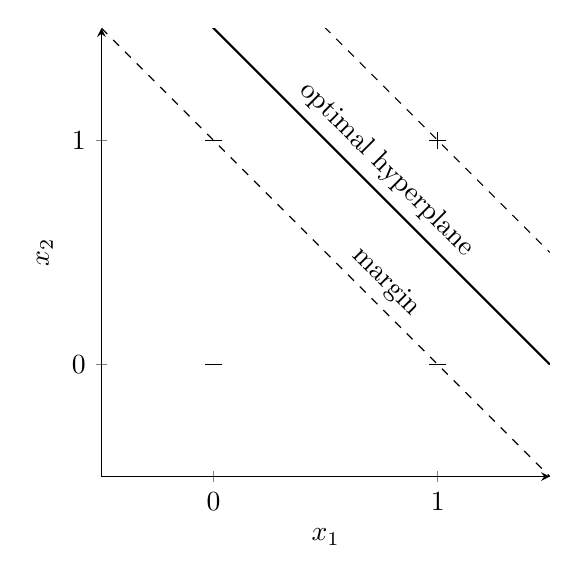
\begin{tikzpicture}
    \begin{axis}[
        axis x line=bottom,
        axis y line=left,
        xlabel={$x_1$},
        ylabel={$x_2$},
        width=0.6\textwidth,
        height=0.6\textwidth,
        xtick={0, 1},
        ytick={0, 1},
        xmin=-0.5, xmax=1.5,
        ymin=-0.5, ymax=1.5,
        domain=-0.5:1.5,
      ]
      \addplot+[only marks, mark=-, color=black, mark size=3pt] coordinates {
        (0, 0) (0, 1) (1, 0)
      };
      \addplot+[only marks, mark=+, color=black, mark size=3pt] coordinates {
        (1, 1)
      };
      \addplot+[mark=none, black, thick] {1.5 - x} node[above, pos=0.6, rotate=-45] {optimal hyperplane};
      \addplot+[mark=none, black, dashed] {1 - x} node[above, pos=0.6, rotate=-45] {margin};
      \addplot+[mark=none, black, dashed] {2 - x};
    \end{axis}
  \end{tikzpicture}
  \tcblower
  The maximal margin classifier generates the hyperplane that maximizes the margin between
  the classes.  In this case, the margin is $\Delta = 0.5$.
\end{figurebox}

Thus, given the training set $(\vec{x}_1, y_1), \dots, (\vec{x}_n, y_n)$, $\vec{x} \in
\mathbb{R}^d$ and $y_i \in \{-1, 1\}$, the optimal hyperplane --- see
\cref{fig:maximal-margin-and} --- is the one that satisfies
\[
  y_i \left[(\vec{w} \cdot \vec{x}_i - b)\right] \geq 1\text{,}
\]
for all $i = 1, \dots, n$ that minimizes $\|\vec{w}\|^2$.  The intuition of the
minimization of the coefficients is that we want only the vectors in the margin to be
exactly equal to $\pm 1$.  (Consequently, the vectors farther from the margin have values
greater than $1$ or less than $-1$.)

Without entering into the details of the optimization process, one interesting property of
the maximal margin classifier is that the separating hyperplane is built from the \emph{support vectors}
--- the vectors that are exactly in the margin.  In \cref{fig:maximal-margin-and}, the
support vectors are the points $(1, 0)$, $(0, 1)$, and $(1, 1)$.

In other words, maximal margin classifier is
\[
  f(x) = \sign\left(\sum_{i=1}^{n} y_i a_i \big(\vec{x}_i \cdot x\big) - b\right)\text{,}
\]
for some $b$ and coefficients $a_i > 0$ for the support vectors ($a_i = 0$ otherwise).

In the case that the classes are not linearly separable, the maximal margin classifier can
be extended to the \emph{soft margin classifier}, which sets the empirical risk to a value
greater than zero.

Moreover, since the number of parameters of the maximal margin classifier depends on the
training data (i.e., the number of support vectors), it is a nonparametric model.
Nonparametric models are those in which the number of parameters is not fixed and can grow
as needed to fit the data.  This property becomes more clear when we consider the kernel
trick, which allows the maximal margin classifier to deal with nonlinear problems.
Consult \textcite{Vapnik1999b}\footfullcite{Vapnik1999b} for more details.

\section{Closing remarks}

The \gls{srm} principle is a powerful tool to understand the generalization ability of
learning machines.  The principle not only explains many of the empirical results in
\gls{ml} but also provides a theoretical framework to guide the development of new
learning machines.

Many powerful methods have been proposed in the literature --- e.g., support vector
machines, boosting, and deep learning --- that can deal with complex nonlinear problems.
I encourage the reader to dive into the literature to learn more about these methods and
the theoretical principles behind them.  Some comments about a few methods are given in
\cref{chap:learning-machines}.

% vim: spell spelllang=en
